\begin{frame}{Pointmaps: Geometry as an Image}
  \centering
  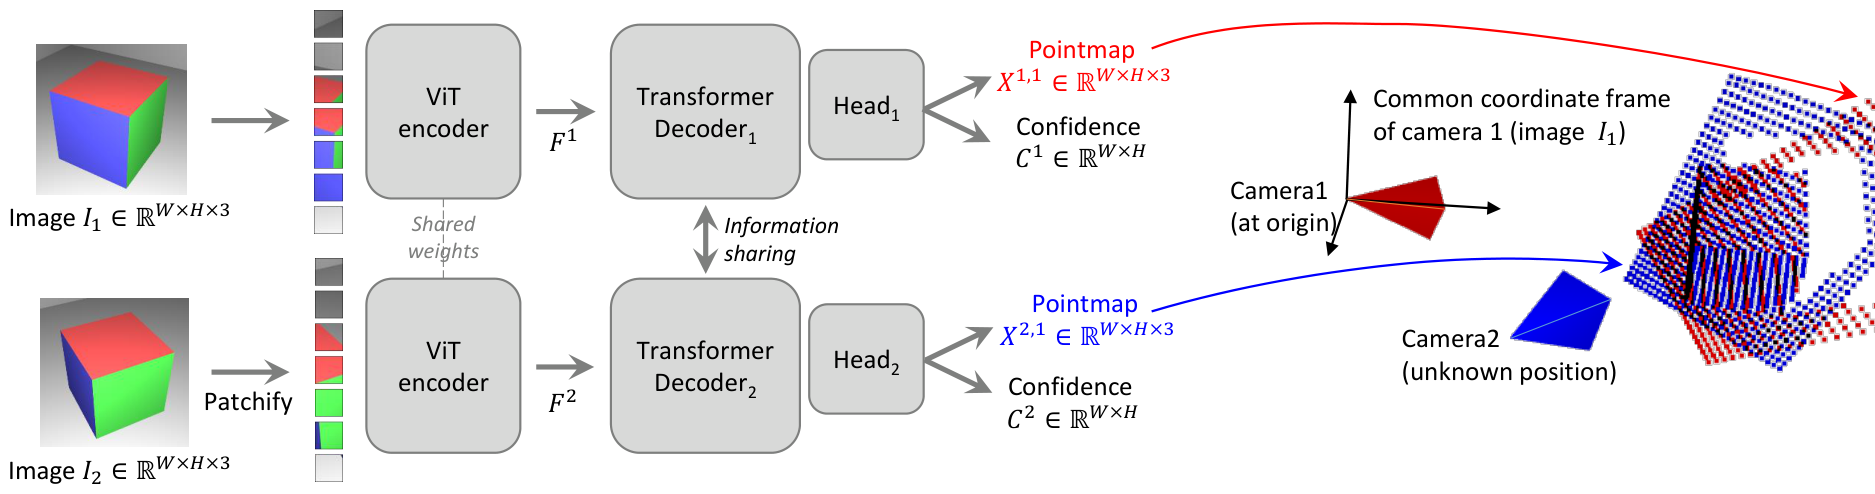
\includegraphics[width=\textwidth,height=0.45\textheight,keepaspectratio]{images/3d-vision/dust3r_fig2_architecture.png}\\[0.2em]
  {\scriptsize Wang et al., ``DUSt3R: Geometric 3D Vision Made Easy,'' CVPR 2024, \href{https://arxiv.org/abs/2312.14132v3}{arXiv:2312.14132v3}, Figure~2.\par}
  \begin{itemize}\footnotesize\itemsep0.3em
    \item \textbf{Pointmap:} an $H\times W\times 3$ array holding, for every pixel, the 3D point it sees, in one chosen camera's frame. With $K$ and depth known it is back-projection, $X(\mathbf{p}) = D(\mathbf{p})\,K^{-1}\tilde{\mathbf{p}}$.
    \item \textbf{Read-outs:} depth is the $Z$ channel; the focal length is the $f$ for which $f\,(X,Y)/Z$ best fits each pixel's offset from the image centre; relative pose comes from Procrustes (a closed-form similarity fit) between image 1's pointmaps from both input orders, or from PnP in RANSAC.
    \item \textbf{DUSt3R:} two images in, with no intrinsics or poses; out: pointmaps $X^{1,1}, X^{2,1}$, both in camera 1's frame, and confidence maps $C^{1,1}, C^{2,1}$.
  \end{itemize}
\end{frame}

\begin{frame}{DUSt3R: Architecture and Confidence-Aware Loss}
  \begin{columns}[T,onlytextwidth]
    \column{0.44\textwidth}
      \begin{itemize}\footnotesize\itemsep0.3em
        \item \textbf{Encoder:} both images pass through one shared (Siamese) ViT-Large, giving token sets $F^1$ and $F^2$.
        \item \textbf{Decoders:} two ViT-Base decoders, one per view. Every block applies self-attention within its view, then cross-attention to the other view, then an MLP, so the two branches exchange information throughout.
        \item \textbf{Heads:} a DPT head per view regresses the pointmap and its confidence map.
        \item \textbf{Confidence without labels:} $C = 1+\exp\tilde{C} > 1$. With $\ell$ the regression error, the per-pixel term is smallest at $C=\alpha/\ell$ when $\ell<\alpha$, and keeps falling toward $C\to1$ when $\ell\geq\alpha$, so confidence tracks inverse error (plot). Since $C>1$, the network must still extrapolate in hard regions, such as areas seen by one view only.
      \end{itemize}
      \vspace{0.2em}
      {\scriptsize Wang et al., CVPR 2024, \href{https://arxiv.org/abs/2312.14132v3}{arXiv:2312.14132v3}, Sections~3.1--3.2 and~4, Eqs.~2--4.\par}
    \column{0.54\textwidth}
      \begin{itemize}\footnotesize\itemsep0.3em
        \setlength{\abovedisplayskip}{3pt}\setlength{\belowdisplayskip}{3pt}
        \item \textbf{Confidence-aware regression loss:}
        \[ \mathcal{L}_{\text{conf}} = \sum_{v\in\{1,2\}} \sum_{i\in\mathcal{D}^v} C_i^{v,1}\Big\lVert \tfrac{1}{z}X_i^{v,1} - \tfrac{1}{\bar{z}}\bar{X}_i^{v,1}\Big\rVert - \alpha\log C_i^{v,1} \]
        $X^{n,m}$: pointmap of image $n$ in camera $m$'s frame; $\bar{X}$: ground truth; $\mathcal{D}^v$: pixels of view $v$ with ground truth; $z$, $\bar{z}$: mean distance of the valid predicted and ground-truth points to the origin, which removes the unknown scale; $\alpha$: regularizer weight.
      \end{itemize}
      \vspace{0.2em}
      \centering
      % Curves computed in Python for alpha = 1: C*l - ln C on C = 1..6 in steps of 0.25.
      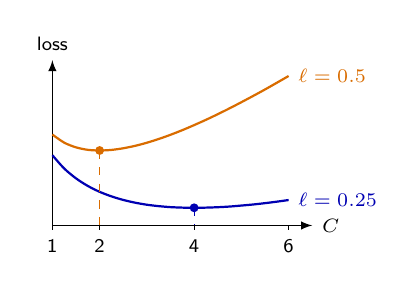
\begin{tikzpicture}[font=\sffamily\scriptsize, >=latex, x=0.6cm, y=1.05cm]
        \draw[->] (1,-0.6) -- (6.5,-0.6) node[right] {$C$};
        \draw[->] (1,-0.6) -- (1,1.4) node[above] {loss};
        \foreach \c in {1,2,4,6} \draw (\c,-0.6) -- (\c,-0.66) node[below] {\c};
        \draw[thick, blue!70!black] plot[smooth] coordinates {(1.00,0.250) (1.25,0.089) (1.50,-0.030) (1.75,-0.122) (2.00,-0.193) (2.25,-0.248) (2.50,-0.291) (2.75,-0.324) (3.00,-0.349) (3.25,-0.366) (3.50,-0.378) (3.75,-0.384) (4.00,-0.386) (4.25,-0.384) (4.50,-0.379) (4.75,-0.371) (5.00,-0.359) (5.25,-0.346) (5.50,-0.330) (5.75,-0.312) (6.00,-0.292)};
        \draw[thick, orange!85!black] plot[smooth] coordinates {(1.00,0.500) (1.25,0.402) (1.50,0.345) (1.75,0.315) (2.00,0.307) (2.25,0.314) (2.50,0.334) (2.75,0.363) (3.00,0.401) (3.25,0.446) (3.50,0.497) (3.75,0.553) (4.00,0.614) (4.25,0.678) (4.50,0.746) (4.75,0.817) (5.00,0.891) (5.25,0.967) (5.50,1.045) (5.75,1.126) (6.00,1.208)};
        \draw[dashed, blue!70!black] (4,-0.386) -- (4,-0.6);
        \draw[dashed, orange!85!black] (2,0.307) -- (2,-0.6);
        \fill[blue!70!black] (4,-0.386) circle (1.6pt);
        \fill[orange!85!black] (2,0.307) circle (1.6pt);
        \node[right, blue!70!black] at (6,-0.29) {$\ell=0.25$};
        \node[right, orange!85!black] at (6,1.21) {$\ell=0.5$};
      \end{tikzpicture}\\[0.1em]
      {\scriptsize Per-pixel term $C\ell-\alpha\log C$ for $\alpha=1$, computed for this slide: both errors are below $\alpha$, so the best $C$ is $\alpha/\ell$, lower for the larger error.\par}
  \end{columns}
\end{frame}

\begin{frame}{CroCo: Pretraining by Cross-View Completion}
  \centering
  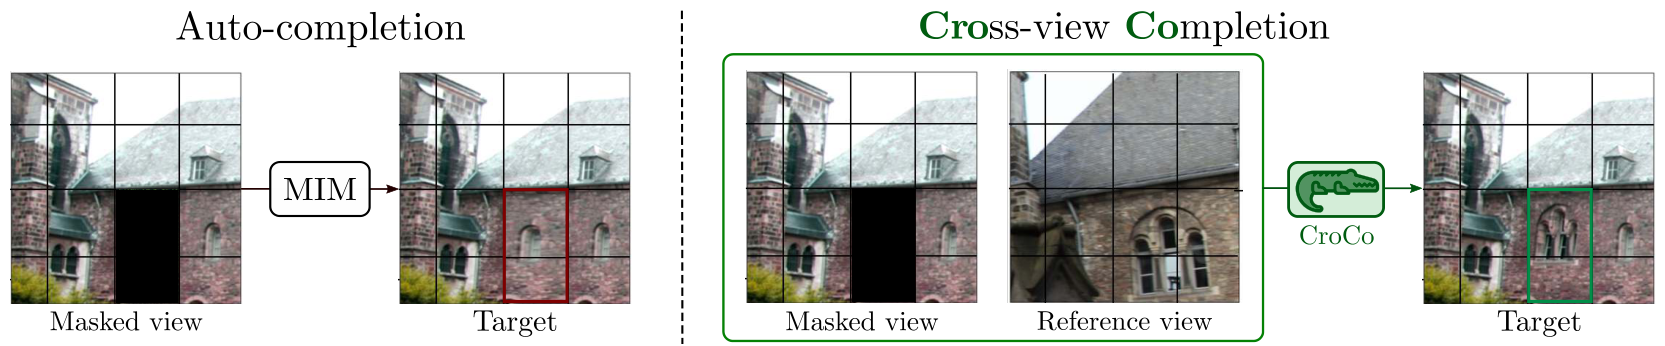
\includegraphics[width=\textwidth,height=0.40\textheight,keepaspectratio]{images/3d-vision/croco_fig1_cross_view_completion.png}\\[0.2em]
  {\scriptsize Weinzaepfel et al., ``CroCo: Self-Supervised Pre-training for 3D Vision Tasks by Cross-View Completion,'' NeurIPS 2022, \href{https://arxiv.org/abs/2210.10716v2}{arXiv:2210.10716v2}, Figure~1.\par}
  \vspace{0.1em}
  \begin{itemize}\footnotesize\itemsep0.3em
    \item \textbf{Left, auto-completion:} masked image modelling as in MAE. The visible patches alone leave the hidden content ambiguous, so the model leans on high-level semantics.
    \item \textbf{Right, cross-view completion:} the decoder also attends, through cross-attention, to a second, unmasked view of the same scene. With 90\% of view 1's patches masked, that view resolves the ambiguity, provided the model relates the two viewpoints.
    \item \textbf{Use in DUSt3R:} its network is inspired by this layout, with one decoder per view so that each view cross-attends to the other, and starts training from CroCo~v2 weights (Weinzaepfel et al., ICCV 2023, \href{https://arxiv.org/abs/2211.10408v3}{arXiv:2211.10408v3}).
  \end{itemize}
\end{frame}

\begin{frame}{Global Alignment: From Pairs to Scenes}
  \begin{itemize}\footnotesize\itemsep0.35em
    \setlength{\abovedisplayskip}{4pt}\setlength{\belowdisplayskip}{4pt}
    \item \textbf{Pair graph:} images are vertices and overlapping pairs are edges $e=(n,m)\in\mathcal{E}$, found by image retrieval, or by running all pairs (about 40\,ms each on an H100) and keeping the confident ones. The network predicts every edge.
    \item \textbf{Objective:} one world-frame pointmap $\chi^n$ per image, and one rigid transform $T_e\in SE(3)$ and one scale $\sigma_e>0$ per pair, subject to $\prod_e\sigma_e=1$, which rules out the trivial $\sigma_e=0$:
    \[ \chi^{*} = \operatorname*{arg\,min}_{\chi,T,\sigma} \sum_{e\in\mathcal{E}} \sum_{v\in e} \sum_{i=1}^{HW} C_i^{v,e}\, \big\lVert \chi_i^{v} - \sigma_e T_e X_i^{v,e} \big\rVert \]
    $X^{v,e}, C^{v,e}$: pair $e$'s pointmap and confidence for image $v$, both in the frame of image $n$, so one transform per pair aligns both of its pointmaps.
    \item \textbf{Cameras from the same problem:} writing $\chi^n(\mathbf{p}) = T_n^{-1}\big(D^n(\mathbf{p})\,K_n^{-1}\tilde{\mathbf{p}}\big)$ returns poses $T_n$, intrinsics $K_n$ and depth maps $D^n$. The residual is a 3D distance, where bundle adjustment uses 2D reprojection error; gradient descent converges in a few hundred steps, seconds on one GPU.
    \item \textbf{Limits:} with all pairs the network runs $N(N-1)/2$ times (45 for 10 images), and the alignment is an offline optimization. Later work reports that it assumes a static scene and that DUSt3R runs out of memory beyond 32 frames (CUT3R and VGGT).
  \end{itemize}
  \vspace{0.2em}
  {\scriptsize Wang et al., CVPR 2024, \href{https://arxiv.org/abs/2312.14132v3}{arXiv:2312.14132v3}, Section~3.4, Eq.~5; static scene: \href{https://arxiv.org/abs/2501.12387v1}{arXiv:2501.12387v1}, Section~4.1; 32 frames: \href{https://arxiv.org/abs/2503.11651v1}{arXiv:2503.11651v1}, Figure~3.\par}
\end{frame}

\begin{frame}{MASt3R: Matching Grounded in 3D}
  \centering
  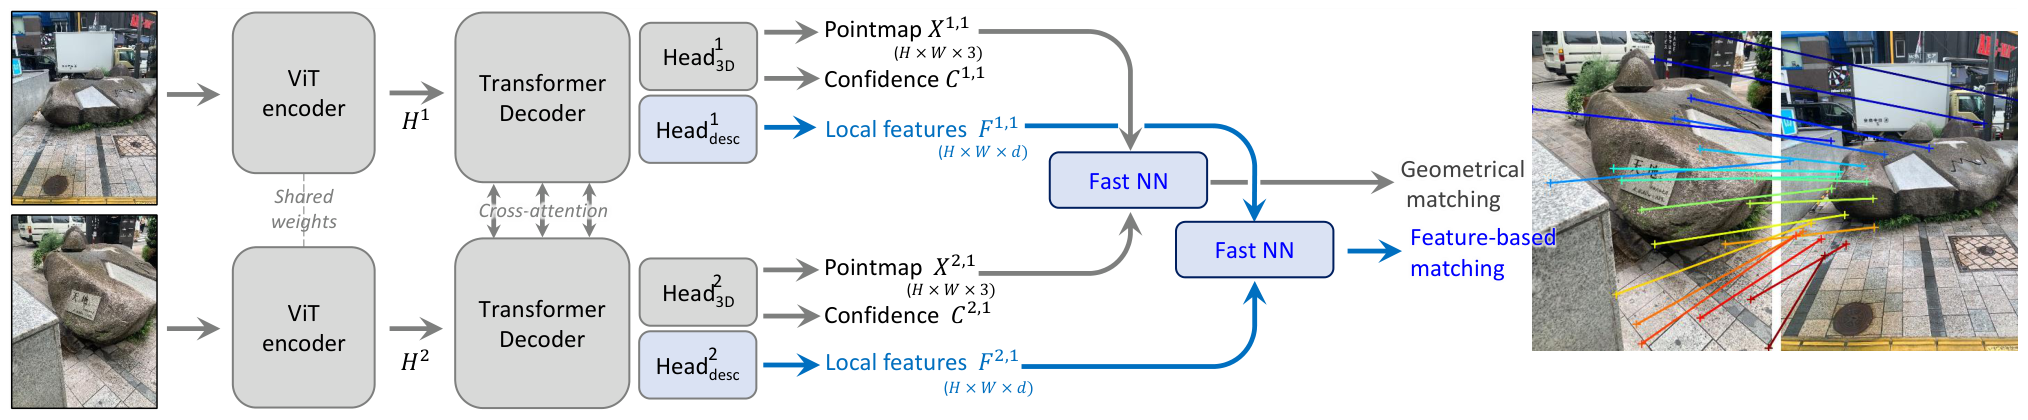
\includegraphics[width=\textwidth,height=0.32\textheight,keepaspectratio]{images/3d-vision/mast3r_fig2_overview.png}\\[0.2em]
  {\scriptsize New parts in blue. Leroy et al., ``Grounding Image Matching in 3D with MASt3R,'' ECCV 2024, \href{https://arxiv.org/abs/2406.09756v1}{arXiv:2406.09756v1}, Figure~2.\par}
  \begin{itemize}\footnotesize\itemsep0.1em
    \item \textbf{Descriptor head:} dense descriptors per image ($H\times W\times d$, $d=24$), trained with an InfoNCE loss: each ground-truth match must pick out its partner among the other image's candidate pixels, a classification in which a nearby pixel earns nothing.
    \item \textbf{Metric pointmaps:} no rescaling on metric ground truth (10 of 14 training sets): scale is learned.
    \item \textbf{Fast reciprocal matching:} from $k$ grid pixels, hop to the nearest descriptor in the other image and back. Pixels that return to their start form reciprocal pairs; the rest repeat the hops from where they landed, and nearly all converge within 5 rounds. $O(kWH)$ work instead of $O(W^2H^2)$.
    \item \textbf{Map-free relocalization} (one reference image, no map): VCRE AUC 0.933, against 0.697 for DUSt3R and 0.634 for the best other published method (the authors' ``30\% (absolute improvement)''). VCRE: virtual correspondence reprojection error, accepted below 90 pixels; AUC: area under the curve.
  \end{itemize}
\end{frame}

\begin{frame}{MASt3R-SLAM: Dense SLAM on Two-View Priors}
  \centering
  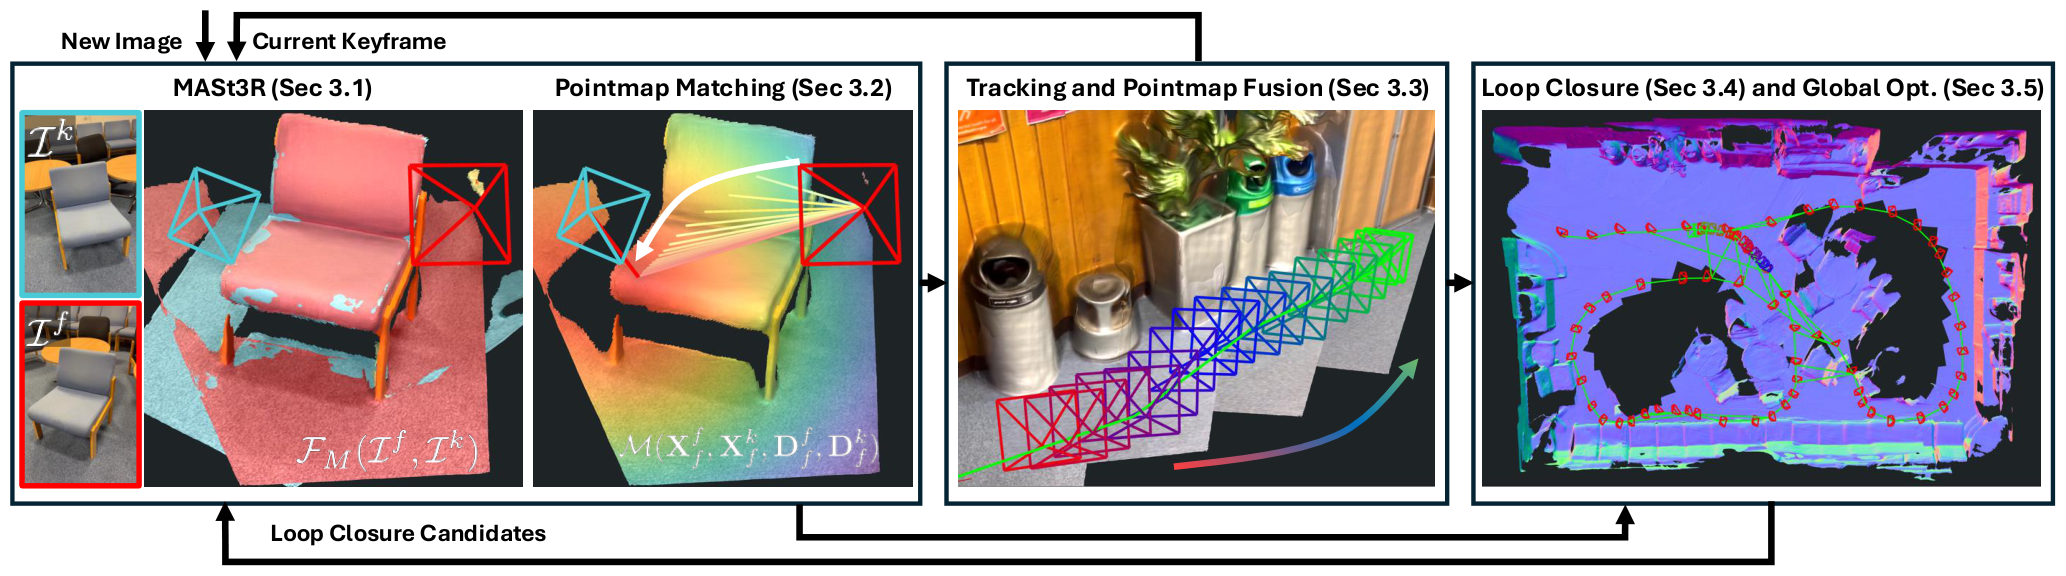
\includegraphics[width=\textwidth,height=0.47\textheight,keepaspectratio]{images/3d-vision/mast3rslam_fig3_system_diagram.png}\\[0.2em]
  {\scriptsize Murai et al., ``MASt3R-SLAM: Real-Time Dense SLAM with 3D Reconstruction Priors,'' CVPR 2025, \href{https://arxiv.org/abs/2412.12392v2}{arXiv:2412.12392v2}, Figure~3.\par}
  \begin{columns}[T,onlytextwidth]
    \column{0.49\textwidth}
      \begin{itemize}\scriptsize\itemsep0.25em
        \item \textbf{Idea:} real-time dense monocular SLAM built bottom-up on MASt3R's two-view predictions; about 15 frames per second on one RTX 4090.
        \item \textbf{Camera model:} only a ``generic central camera'', all rays through one centre. Each pointmap, normalized to unit rays, defines its own camera, so a changing zoom needs no calibration. Strong lens distortion still degrades MASt3R's predictions; the EuRoC images were undistorted first.
      \end{itemize}
    \column{0.49\textwidth}
      \begin{itemize}\scriptsize\itemsep0.25em
        \item \textbf{Front-end:} matching by iterative projection onto these rays (2\,ms, against 2\,s for MASt3R's dense matching), tracking against the current keyframe with a ray error, and pointmap fusion per keyframe. Poses live in Sim(3) because scale varies between predictions.
        \item \textbf{Back-end:} loop-closure candidates from retrieval on MASt3R encoder features, then Gauss--Newton optimization of all keyframe poses in Sim(3).
      \end{itemize}
  \end{columns}
\end{frame}

\begin{frame}{VGGT: One Transformer, Many 3D Outputs}
  \centering
  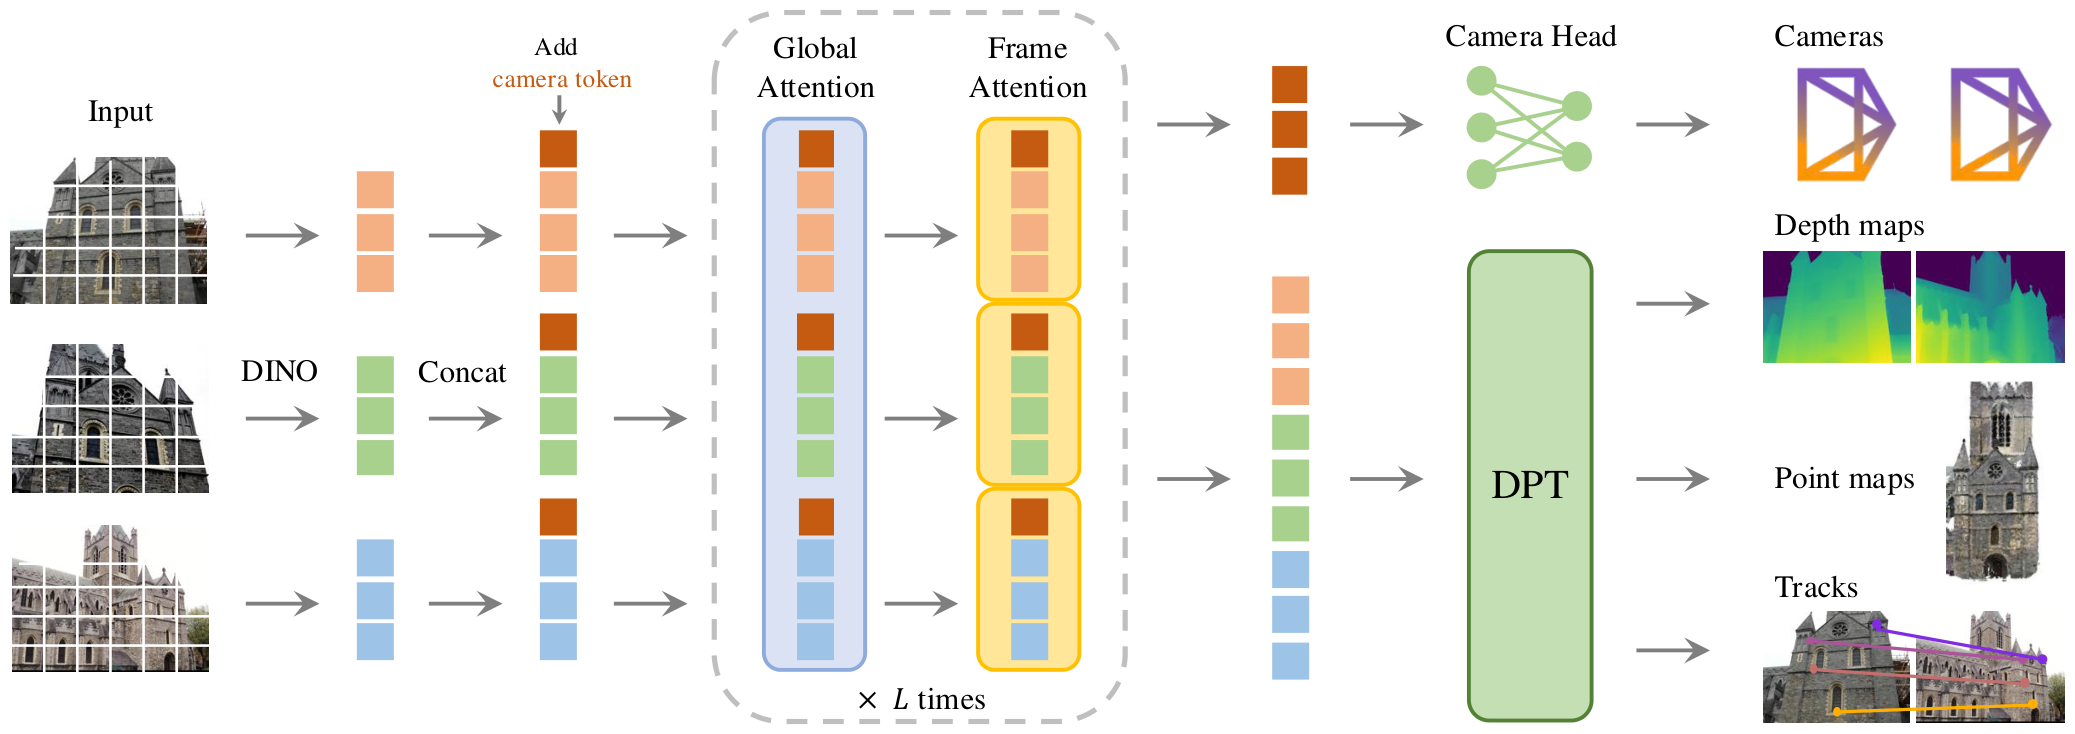
\includegraphics[width=\textwidth,height=0.45\textheight,keepaspectratio]{images/3d-vision/vggt_fig2_architecture.png}\\[0.2em]
  {\scriptsize Wang et al., ``VGGT: Visual Geometry Grounded Transformer,'' CVPR 2025 (Best Paper Award), \href{https://arxiv.org/abs/2503.11651v1}{arXiv:2503.11651v1}, Figure~2.\par}
  \begin{columns}[T,onlytextwidth]
    \column{0.49\textwidth}
      \begin{itemize}\scriptsize\itemsep0.2em
        \item \textbf{Input:} one, a few, or hundreds of images. DINOv2 turns each frame into patch tokens, plus one camera token and four register tokens (extra learned tokens that collect global information and are discarded at the output); frame 1 has its own learned tokens, so every output is in camera 1's frame.
        \item \textbf{Heads:} camera head: quaternion, translation and field of view (principal point centred); DPT head: depth maps and pointmaps with uncertainty, and features for point tracks (the pixel positions of one scene point across all frames).
      \end{itemize}
    \column{0.49\textwidth}
      \begin{itemize}\scriptsize\itemsep0.2em
        \item \textbf{Alternating attention:} $L=24$ blocks, each with a frame-wise and a global self-attention layer; no cross-attention. About 1.2 billion parameters.
        \item \textbf{Speed:} about 0.2\,s for 10 frames on one H100, against 7--9\,s for DUSt3R and MASt3R with global alignment. With optional BA the total is 1.8\,s, and pose AUC@30 (accuracy integrated up to 30$^\circ$ of error) on RealEstate10K (about 80K YouTube clips with SLAM-derived poses) rises from 85.3 to 93.5.
      \end{itemize}
  \end{columns}
\end{frame}

\begin{frame}{Feed-Forward 3D Models of 2025--2026}
  \centering
  {\scriptsize\setlength{\tabcolsep}{4pt}
  \begin{tabular}{>{\raggedright\arraybackslash}p{1.6cm} >{\raggedright\arraybackslash}p{1.3cm} >{\raggedright\arraybackslash}p{2.0cm} >{\raggedright\arraybackslash}p{2.8cm} >{\raggedright\arraybackslash}p{4.7cm}}
    \toprule
    \textbf{Model} & \textbf{Venue} & \textbf{Input} & \textbf{Output} & \textbf{Key idea} \\
    \midrule
    CUT3R & CVPR 2025 & video or photo collection, static or dynamic & metric pointmap and camera per frame, in one shared frame & a recurrent state is read and updated with each new frame: online, no global alignment \\
    \addlinespace[0.1em]
    $\pi^3$ & ICLR 2026 & images in any order & per-view pose and local pointmap, up to one similarity & permutation-equivariant: no reference view, no frame-index embedding \\
    \addlinespace[0.1em]
    MapAnything & 3DV 2026 & images, plus intrinsics, poses or depth if known & up-to-scale depth, ray directions and poses, plus one metric scale & factored output; one model for more than 12 tasks: SfM, localization, multi-view stereo (dense depth from posed images) \\
    \addlinespace[0.1em]
    Depth Anything 3 & ICLR 2026 & any number of images, posed or not & depth and a per-pixel ray (origin and direction) & a plain DINOv2 transformer with cross-view attention; teacher--student training \\
    \addlinespace[0.1em]
    VGGT-$\Omega$ & CVPR 2026 & static and dynamic sequences & cameras and depth maps & register attention (frames interact only via register tokens) in 25\% of global layers; up to 10B parameters \\
    \bottomrule
  \end{tabular}\par}
  \begin{itemize}\scriptsize\itemsep0.1em
    \item \textbf{Reported gains}, on the authors' own evaluations: $\pi^3$ runs at 57.4 frames per second against 43.2 for VGGT (KITTI, one A800 GPU); Depth Anything 3 beats VGGT by 35.7\% in pose and 23.6\% in geometric accuracy on average; VGGT-$\Omega$ reaches a camera AUC@3 of 40.0 on Sintel (synthetic, with large moving objects), against 22.5 for the previous best.
  \end{itemize}
  {\scriptsize CUT3R: Wang et al., \href{https://arxiv.org/abs/2501.12387v1}{arXiv:2501.12387v1}; $\pi^3$: Wang et al., \href{https://arxiv.org/abs/2507.13347v3}{arXiv:2507.13347v3}; MapAnything: Keetha et al., \href{https://arxiv.org/abs/2509.13414v3}{arXiv:2509.13414v3}; Depth Anything 3: Lin et al., \href{https://arxiv.org/abs/2511.10647v1}{arXiv:2511.10647v1}; VGGT-$\Omega$: Wang et al., \href{https://arxiv.org/abs/2605.15195v1}{arXiv:2605.15195v1}.\par}
\end{frame}

\begin{frame}{Classical Pipeline vs Feed-Forward Models}
  \centering
  {\footnotesize\setlength{\tabcolsep}{4pt}
  \begin{tabular}{>{\raggedright\arraybackslash}p{2.0cm} >{\raggedright\arraybackslash}p{5.0cm} >{\raggedright\arraybackslash}p{5.6cm}}
    \toprule
     & \textbf{Classical (SfM or SLAM, BA)} & \textbf{Feed-forward (DUSt3R to VGGT-$\Omega$)} \\
    \midrule
    Inputs & overlapping, textured images; intrinsics known or refined in BA & images only; MapAnything also accepts intrinsics, poses or depth, Depth Anything 3 known poses \\
    \addlinespace[0.3em]
    Outputs & poses and sparse points; dense depth needs multi-view stereo & poses, intrinsics, dense depth or pointmaps; one forward pass from VGGT on \\
    \addlinespace[0.3em]
    Speed, 10 images & COLMAP with SuperPoint and SuperGlue: about 15\,s & VGGT 0.2\,s; DUSt3R or MASt3R with global alignment 7--9\,s (all on one H100) \\
    \addlinespace[0.3em]
    Metric scale & one camera: up to a similarity; scale from an IMU or known sizes & learned: MASt3R, CUT3R, MapAnything metric; DUSt3R, VGGT, $\pi^3$ up to scale \\
    \addlinespace[0.3em]
    Accuracy, AUC@10 & on IMC (Image Matching Challenge): COLMAP with SIFT 44.79, up to 72.19 with learned matches; VGGSfMv2 (learned, with differentiable BA) 76.82 & VGGT alone 71.26; streaming models trail optimization on MASt3R outputs \\
    \bottomrule
  \end{tabular}\par}
  \vspace{0.5em}
  {\scriptsize VGGT: \href{https://arxiv.org/abs/2503.11651v1}{arXiv:2503.11651v1}, Tables~1 and~10; MapAnything: \href{https://arxiv.org/abs/2509.13414v3}{arXiv:2509.13414v3}, Section~2; the other models are cited on the previous slides.\par}
\end{frame}

\begin{frame}{Failure Modes and Combining Both Approaches}
  \centering
  {\footnotesize\setlength{\tabcolsep}{4pt}
  \begin{tabular}{>{\raggedright\arraybackslash}p{2.0cm} >{\raggedright\arraybackslash}p{5.0cm} >{\raggedright\arraybackslash}p{5.6cm}}
    \toprule
     & \textbf{Classical (SfM or SLAM, BA)} & \textbf{Feed-forward (DUSt3R to VGGT-$\Omega$)} \\
    \midrule
    Many images & sparse BA and pose graphs keep large maps consistent & VGGT backbone on one H100: 8.75\,s and 40.6\,GB for 200 frames; CUT3R may drift on very long sequences \\
    \addlinespace[0.3em]
    Dynamic scenes & assume a static scene; large moving objects are hard & CUT3R, $\pi^3$, VGGT-$\Omega$ train on dynamic data; VGGT fails on substantial non-rigid deformation \\
    \addlinespace[0.3em]
    Unusual inputs & few views, little camera motion, non-Lambertian surfaces & outside the training data: fisheye, extreme rotation, motion blur, sudden zoom; transparent objects, since light transport is not modelled ($\pi^3$) \\
    \bottomrule
  \end{tabular}\par}
  \begin{itemize}\footnotesize\itemsep0.3em
    \item \textbf{Combine them:} feed-forward output initializes, optimization refines. VGGT's cameras, points and point tracks start BA without triangulation, raising IMC AUC@10 from 71.26 to 84.91.
    \item MASt3R-SLAM wraps two-view MASt3R predictions in a keyframe SLAM back-end with loop closure and Sim(3) optimization, at about 15 frames per second.
  \end{itemize}
  \vspace{0.2em}
  {\scriptsize VGGT \href{https://arxiv.org/abs/2503.11651v1}{arXiv:2503.11651v1}, Tables~9--10, Section~5; CUT3R \href{https://arxiv.org/abs/2501.12387v1}{arXiv:2501.12387v1}, Sections~4.2 and~5; VGGT-$\Omega$ \href{https://arxiv.org/abs/2605.15195v1}{arXiv:2605.15195v1}, Supplement~C; $\pi^3$ \href{https://arxiv.org/abs/2507.13347v3}{arXiv:2507.13347v3}, Appendix~A.8; DUSt3R \href{https://arxiv.org/abs/2312.14132v3}{arXiv:2312.14132v3}, Section~1; MASt3R-SLAM \href{https://arxiv.org/abs/2412.12392v2}{arXiv:2412.12392v2}.\par}
\end{frame}
